\documentclass[12pt]{article}
\usepackage[margin=2.5cm]{geometry}
\usepackage{enumerate}
\usepackage{amsfonts}
\usepackage{amsmath}
\usepackage{fancyhdr}
\usepackage{amsmath}
\usepackage{amssymb}
\usepackage{amsthm}
\usepackage{mdframed}
\usepackage{graphicx}
\usepackage{subcaption}
\usepackage{adjustbox}
\usepackage{listings}
\usepackage{xcolor}
\usepackage{courier}
\usepackage[utf]{kotex}
\usepackage{hyperref}
\usepackage{soul}

\definecolor{codegreen}{rgb}{0,0.6,0}
\definecolor{codegray}{rgb}{0.5,0.5,0.5}
\definecolor{codepurple}{rgb}{0.58,0,0.82}
\definecolor{backcolour}{rgb}{0.95,0.95,0.92}

\lstdefinestyle{mystyle}{
    backgroundcolor=\color{backcolour},
    commentstyle=\color{codegreen},
    keywordstyle=\color{magenta},
    numberstyle=\tiny\color{codegray},
    stringstyle=\color{codepurple},
    basicstyle=\ttfamily\footnotesize,
    breakatwhitespace=false,
    breaklines=true,
    captionpos=b,
    keepspaces=true,
    numbers=left,
    numbersep=5pt,
    showspaces=false,
    showstringspaces=false,
    showtabs=false,
    tabsize=1
}

\lstset{style=mystyle}

\pagestyle{fancy}
\renewcommand{\headrulewidth}{0.4pt}
\lhead{CSC 369}
\rhead{Midterm 4 Solution}

\begin{document}
\title{CSC 369 Midterm 4 Solution}

\bigskip

\begin{enumerate}[1.]
    \item

    \begin{enumerate}[a)]

        \item
        \begin{enumerate}[1)]
            \item 4 - inode blocks. 1 for the file \texttt{c}, and 3 for the
            directdories \texttt{/}, \texttt{a}, \texttt{b}

            \item 3 - directory blocks - one for root \texttt{/}, one for \texttt{a},
            the other for \texttt{b}

            \item 1 - single indirect block as far as we know. The file definitely has more than
            12 blocks (\# of data blocks pointed by direct pounters), but less than 1036 (\# of data blocks pointed
            by direct pointers and single indirect pointers). We are reading block 1034.

            \item 1 - data block for file \texttt{c}
        \end{enumerate}

        \item

        All of the above

        \bigskip

        \underline{\textbf{Notes}}

        \begin{itemize}
            \item \textbf{Inode}

            \begin{center}
            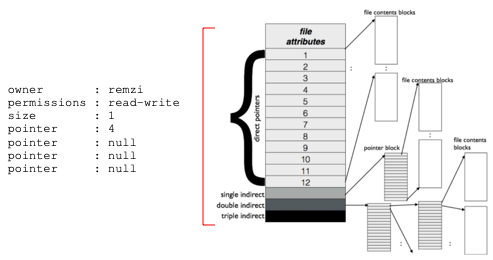
\includegraphics[width=0.6\linewidth]{../images/midterm_4_solution_1.png}
            \end{center}

            \begin{itemize}
                \item Is short form of \textbf{index node}
                \item Describes a file system object such as file or data
                \item Contains all information about a file/directory, including
                \begin{itemize}
                    \item File Type,
                    \item Size
                    \item Number of blocks allocated to it
                    \item Protection information
                    \item Time information (e.g time created, time modified)
                    \item Location of data blocks residing on disk
                \end{itemize}

            \end{itemize}
        \end{itemize}

        \bigskip

        \underline{\textbf{References}}

        \begin{enumerate}[1)]
            \item Wikipedia, Inode, \href{https://en.wikipedia.org/wiki/Inode}{link}
            \item Machanick, Philip. (2016). Teaching Operating Systems: Just Enough Abstraction. 642. 10.1007/978-3-319-47680-3\_10., \href{https://www.researchgate.net/figure/Conceptual-index-node-inode-The-top-level-block-contains-file-attributes-12-direct_fig1_306347325}{link}
        \end{enumerate}

        \item

        Size, the location of data blocks that reside on disk

        \bigskip

        \underline{\textbf{Notes}}

        \begin{itemize}
            \item I wonder what information about blocks inode has. Is it total number
            of blocks both inode and data, or just data?
            \item I struggled a bit on this one. I should find an easier way to
            remember which information inode has
        \end{itemize}

        \item

        \bigskip

        \underline{\textbf{Notes}}

        \begin{itemize}
            \item I wonder how system call for reading file in UNIX works. Does it check for bitmap?
            \item I wonder how system call for deleting file in UNIX works
            \item I wonder how system call for adding file in UNIX works
            \item \textbf{Creash Scenarios}

            \begin{itemize}
                \item When only new data block is written to disk

                \begin{itemize}
                    \item This is fine in system's point of view
                    \item No inode points to it (it doesn't contain any information about file)
                    \item No bitmap points to it
                    \item Is as if write never occured
                \end{itemize}
                \item When only the updated inode is written to disk
                \begin{itemize}
                    \item There is no bitmap that's pointing to it
                    \item There is new inode where existing inode is
                    \item The data block \texttt{Db} hasn't been created
                    \item Reading data where \texttt{Db} is will return garbage data
                    \item there is a term for this. Is called \textbf{File-System inconsistency}
                \end{itemize}
                \item When only inode bitmap is written to disk
                \item When only data bitmap is written to disk
            \end{itemize}
        \end{itemize}

    \end{enumerate}
\end{enumerate}


\end{document}